\documentclass[12pt]{article}
\usepackage{polski}
\usepackage[utf8]{inputenc}
\usepackage[T1]{fontenc}
\usepackage{amsmath}
\usepackage{amsfonts}
\usepackage{fancyhdr}
\usepackage{lastpage}
\usepackage{multirow}
\usepackage{amssymb}
\usepackage{amsthm}
\usepackage{textcomp}
\frenchspacing
\usepackage{fullpage}
\setlength{\headsep}{30pt}
\setlength{\headheight}{12pt}
%\setlength{\voffset}{-30pt}
%\setlength{\textheight}{730pt}
\pagestyle{myheadings}
%\usepackage{kuvio,amscd,diagrams,dcpic,xymatrix,diagxy}
\usepackage{tikz,paralist,mathtools}
\usetikzlibrary{matrix,arrows,decorations}

\DeclareMathOperator{\coker}{coker}
\DeclareMathOperator{\Hom}{Hom}
\DeclareMathOperator{\Tor}{Tor}
\DeclareMathOperator{\Mor}{Mor}
\DeclareMathOperator{\Kom}{Kom}
\DeclareMathOperator{\sgn}{sgn}
\DeclareMathOperator{\Ext}{Ext}
\DeclareMathOperator{\Ob}{Ob}
\DeclareMathOperator{\Cone}{C}
\DeclareMathOperator{\Cyl}{Cyl}
\DeclareMathOperator{\Der}{D}
\DeclareMathOperator{\K}{K}
\newcommand{\Set}{\mathrm{Set}}
\newcommand{\Top}{\mathrm{Top}}
\newcommand{\Rmod}{\mathrm{R-mod}}
\newcommand{\id}{\mathrm{id}}
\newcommand{\A}{\mathcal{A}}
\newcommand{\B}{\mathcal{B}}
\newcommand{\C}{\mathcal{C}}
\newcommand{\D}{\mathcal{D}}
\newcommand{\Q}{\mathcal{Q}}
\newcommand{\qi}{quasi-isomorphism}

\newcommand{\bigslant}[2]{{\left.\raisebox{.2em}{$#1$}\middle/\raisebox{-.2em}{$#2$}\right.}}
\newcommand{\mf}[1]{{\mathfrak{#1}}}
\newcommand{\mb}[1]{{\mathbb{#1}}}
\newcommand{\mc}[1]{{\mathcal{#1}}}
\newcommand{\mr}[1]{{\mathrm{#1}}}


\newcounter{punkt}

\theoremstyle{plain}
\newtheorem{theorem}[punkt]{Theorem}
\newtheorem{lemma}[punkt]{Lemma}
\newtheorem{definition}[punkt]{Definition}
\newtheorem{fact}[punkt]{Fact}
\newtheorem{proposition}[punkt]{Proposition}
\newtheorem{corollary}[punkt]{Corollary}

\theoremstyle{definition}
\newtheorem{remark}[punkt]{Remark}
\newtheorem{example}[punkt]{Example}
\newtheorem{exercise}[punkt]{Exercise}



\markright{Piotr Suwara\hfill Homological algebra II: 8 September 2014\hfill}

\begin{document}
	$\C$ -- any abelian category.
	
	\begin{definition}[$n$-suspension functor]
		$X \in \Kom(\C)$, then $X[n] \in \Kom(\C)$, $(X[n])_i = X_{n+i}$,
		$d_{X[n]} = (-1)^n d_X$.
		
		$f:X \to Y$, $f[n] : X[n] \to Y[n]$ defined in an obvious way.
		
		$T: \Kom(\C) \to \Kom(\C)$, $T(X) = X[1]$, is called
		a~\emph{translation / shift/ suspension} functor.
	\end{definition}
	
	\begin{definition}
		$\Kom(\C)$ is known already.
		
		$\Kom^+(\C) = \{ X \in \Kom(\C) : \exists_{i_0} \forall_{i \leq i_0} X_i = 0 \}$
		
		$\Kom^-(\C)$ obvious.
		
		$\Kom^b(\C) = \Kom^+(\C) \cap \Kom^-(\C)$
	\end{definition}
	
	\begin{remark}
		$T$ is well defined in each of these.
	\end{remark}
	
	\begin{definition}[cone]
		$f: X \to Y$, $\mr{Cone}(f) = \mr{C}(F)  \in \Kom(\C)$ is the
		\emph{cone} of $f$.
		
		$\Cone(f)_i = X[1]_i \oplus Y_i$, $d_{\Cone(f)} = 
		(-d_X \pi_1, f[1] \pi_1 + d_y \pi_2)$.
	\end{definition}
	
	\begin{definition}[cylinder]
		$f:X \to Y$, $\Cyl(f) \in \Kom(\C)$ is the \emph{cylinder} of $f$.
		
		$\Cyl(f)_i = X_i \oplus X[1]_i \oplus Y_i$, $d_{\Cyl(f)} =
		(d_x \pi_1 - \pi_2, - d_X \pi_2, f[1] \pi_2 + d_Y \pi_3)$.
	\end{definition}
	
	\begin{remark}
		Once in life it is worth to check that $d^2=0$ for the cone and the cylinder.
	\end{remark}
	
	\begin{fact}
		For any $f: X \to Y$ the following diagram has exact rows 
		and is functorial in $f$:
		
		\begin{tikzpicture}
			\matrix(m)[matrix of math nodes, row sep=1em, column sep=1em]
			{ & 0 & Y & \Cone(f) & X[1] & 0 \\
			0 & X & \Cyl(f) & \Cone(f) & 0 & \\
			& X & Y & & & \\};
			\path[->,font=\scriptsize]
			(m-1-2) edge (m-1-3)
			(m-1-3) edge node[auto] {$\pi$} (m-1-4)
			  edge node[auto] {$\alpha$} (m-2-3)
			(m-1-4) edge (m-1-5)
			  edge node[auto] {$=$} (m-2-4)
			(m-1-5) edge (m-1-6)
			(m-2-1) edge (m-2-2)
			(m-2-2) edge node[auto] {$\bar{f}$} (m-2-3)
			  edge node[auto] {$=$} (m-3-2)
			(m-2-3) edge (m-2-4)
			  edge node[auto] {$\beta$} (m-3-3)
			(m-2-4) edge (m-2-5)
			(m-3-2) edge node[auto] {$f$} (m-3-3);
		\end{tikzpicture}
		
		where $ \beta = f \pi_1 + \pi_3$ and other maps are obvious.
		
		Also, $\alpha, \beta$ are \qi, with $\beta \alpha = \id_Y$
		(therefore $Y \sim \Cyl(f)$ in $\Der{\C}$.
	\end{fact}
	
	\begin{definition}[triangle]
		In the category $\Kom(\C)$ a~\emph{triangle} is any sequence
		of the form $X \to Y \to Z \to X[1]$.
		
		A~map of triangles is given by a~commutative diagram
		
		\begin{tikzpicture}
			\matrix(m)[matrix of math nodes, row sep=1em, column sep=1em]
			{ X & Y & Z & X[1] \\
			X' & Y' & Z' & X'[1] \\};
			\path[->,font=\scriptsize]
			(m-1-1) edge (m-1-2)
			  edge node[auto] {$f$} (m-2-1)
			(m-1-2) edge (m-1-3)
			  edge node[auto] {$g$} (m-2-2)
			(m-1-3) edge (m-1-4)
			  edge node[auto] {$h$} (m-2-3)
			(m-1-4) edge node[auto] {$f[1]$} (m-2-4)
			(m-2-1) edge (m-2-2)
			(m-2-2) edge (m-2-3)
			(m-2-3) edge (m-2-4);
		\end{tikzpicture}
		
		A~triangle $X \to Y \to Z \to X[1]$ is distinguished
		if it is isomorphic to a~triangle
		$X' \to \Cyl(f) \to \Cone(f) \to X'[1]$ for some $f:X' \to Y'$.
	\end{definition}
	
	\begin{fact}
		Every exact sequence in $\Kom(\C)$ is quasi-isomorphic 
		to a~sequence $0 \to X \to \Cyl(f) \to C(f) \to 0$.
	\end{fact}
	
	\begin{fact}
		If $X \to Y \to Z \to X[1]$ is distinguished, then
		it induces a~long exact sequence of cohomology groups:
		$\ldots \to H^i(X) \to H^i(Y) \to H^i(Z) \to H^{i+1}(X) \to \ldots$
	\end{fact}
	
	\begin{definition}[homotopy category]
		$\K(\C)$ is the \emph{homotopy category} of $\Kom(\C)$, defined via
		$\Ob(\K(\C)) = \Ob(\Kom(\C))$ and $\Mor_{\K(\C)}(X,Y)
		= \Mor_{\Kom(\C)}(X,Y)/\sim$,
		where $\sim$ is a~chain homotopy relation.
	\end{definition}
	
	\begin{theorem}
		Let $S$ be a~class of {\qi}s in $\K(\C)$. 
		Then $\K(\C)[S^{-1}]$ is isomorphic to $\Der{\C}$ in a~canonical way.
		
		This applies to any of $\Kom^{\ast}(\C)$.
	\end{theorem}
	
	\begin{lemma}
		Assume $f, g: X \to Y$ are chain homotopic in $\Kom(\C)$.
		Then $\Q(f) = \Q(g)$.
	\end{lemma}
	
	\begin{theorem}
		In any of $\K^\ast(\C)$ the class of {\qi}s is localising.
	\end{theorem}
	
	\begin{theorem}
		$\Der{\C}$ is an additive category.
	\end{theorem}
















\end{document}
 
 
